\subsection{Opis}
System zawiera następujące elementy:
\begin{itemize}
	\item Kamera przednia
	\item Kamera tylna
	\item Komputer
	\item Ekran
	\item Głośnik
\end{itemize}

Obraz z kamer przesyłany jest do komputera, gdzie zostaje on przetworzony, oraz przeprowadzany jest proces wykrywania obiektów. Następnie komputer przesyła przetworzony obraz na ekran, oraz może uruchomić sygnał dźwiękowy jeśli wykryty zostanie określony typ obiektu.



\subsection{Schemat}
    \begin{figure}[H]
	\centering
	\resizebox{\columnwidth}{!}{%
		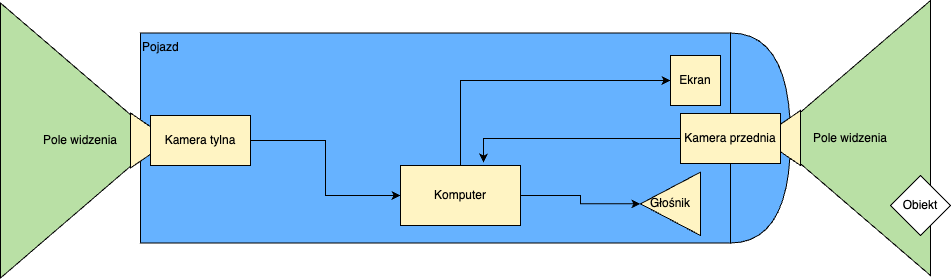
\includegraphics{Img/architektura.png}%
	}
	\caption{Schemat architektury wysokopoziomowej systemu:}
	\label{fig:architektura_diagram}
\end{figure}